\documentclass[dvipdfmx]{article}
\usepackage[dvipdfmx]{graphicx}
\usepackage{amsmath, amssymb}
\usepackage{mathtools}
\usepackage{here}
\usepackage{url}
\begin{document}
\title{Weekly Report}
\author{Riku Gondow}
\date{September 22, 2022}
\maketitle
\section{Progress}
\begin{itemize}
    \item Attend FIT and listen to Prof. Sugiyama's lecture
    \begin{itemize}
        \item Learn theory of weakly supervised learning, transition learning, and noise robust learning. Also learn that there are methods that are theoretically guaranteed to be optimal if the number of data n is increased, other than heuristic methods that do not guarantee a reduction in estimation error.
    \end{itemize}

    \item Continue to implement DDLM\cite{ddlm}
    \begin{itemize}
        \item Send e-mail to the first author of "dipole" paper
        and stop implementation because no reply is expected.
    \end{itemize}

    \item Consider other approachs
    \begin{itemize}
        \item Look over several papers about Person ID using ECG
        and decide to apply the method using ECG to Person ID using radar signals.
    \end{itemize}

    \item Find a new dataset "Medical Radar Signal Dataset for Non-Contact Respiration and Heart Rate Measurement"\cite{dataset}
\end{itemize}

\section{Paper\cite{ensemble}}
This paper proposes a personal identification technique based on an ensemble of LSTM and CNN that uses ECGs. 

\subsection{Method}
\begin{enumerate}
    \item Preprocessing
    \begin{itemize}
        \item remove noises using a low-pass filter
        \item shifts the baseline of the signal above or below the x-axis of the signal
        \item standardize the signals
        \item divide into cycles with respect to R-peaks
    \end{itemize}

    \begin{figure}[H]
        \begin{center}
        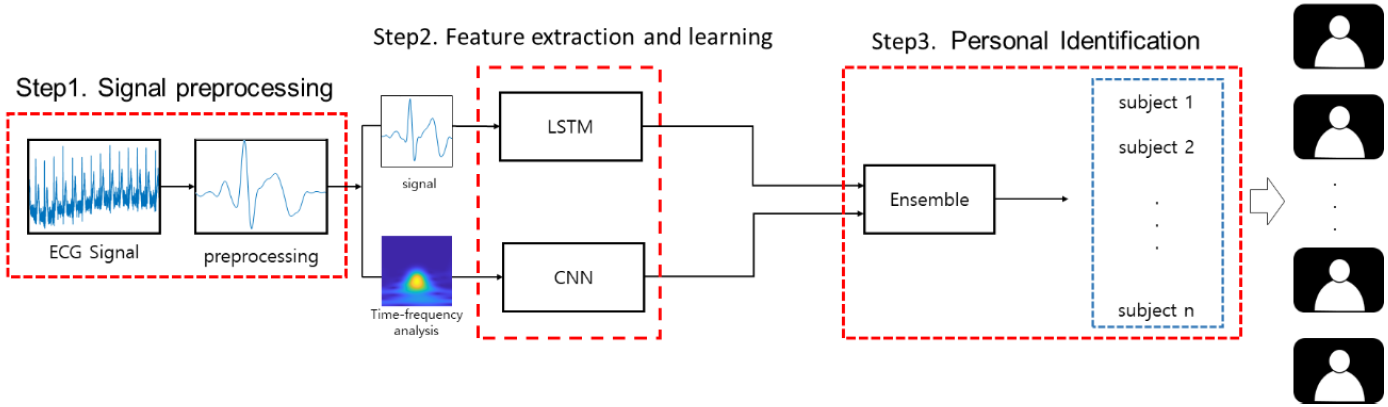
\includegraphics[width=\linewidth]{./img/LSTM-CNN.png}
        \end{center}
        \caption{Overview of ensemble approach of LSTM and 2D-CNN}
    \end{figure}

    \item Feature extraction and learning
    \begin{itemize}
        \item LSTM neural network is used for identifying the sequential information to analyze 1D time-series or sequence signals. To improve the accuracy, LSTM neural network is expanded and finally two LSTM layers are used
        \item ECG signals use 2D images transformed by STFT, scalogram, and FSST through a time–frequency transform. The images expressed through a time–frequency transform are classified with pre-trained CNN models (namely, GoogleNet, VGG-19, and ResNet-101) 
    \end{itemize}
    \item Personal identification \newline
    Simply, an ensemble uses the multiplication of model outputs from LSTM and CNN to determine the results.
\end{enumerate}

\subsection{Result}
\begin{figure}[H]
\begin{center}
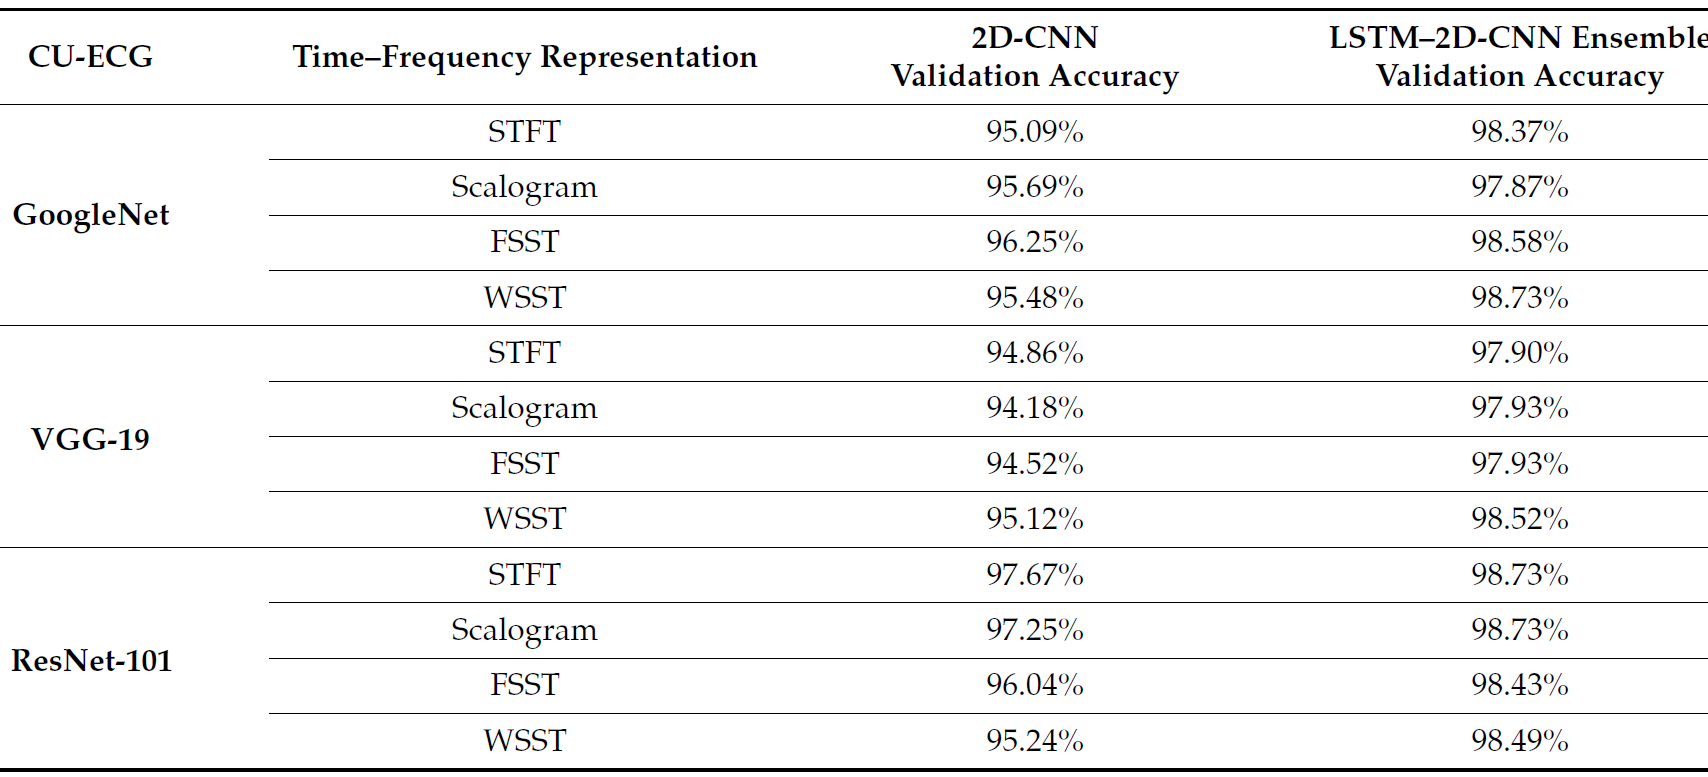
\includegraphics[width=\linewidth]{./img/ensemble_result.png}
\end{center}
\caption{Accuracy of LSTM and 2D-CNN-based ensemble}
\end{figure}

It can be confirmed that the individual identification performance through the ensemble method using the maximum value by multiplying the score values of each model proposed in this paper is superior to the performance of the single model.

The results of two LSTM neural networks showed that the highest performance was 95.12\% when epoch was set at 100 and the minibatch size at 128, and the performance of 2D-CNN was the highest at 97.67\% for ResNet-101. Finally, the performance of each model of LSTM and 2D-CNN was improved by an ensemble method, with a personal identification performance of at least 1.06\% to a maximum of 3.75\% compared to that of a single model.


\section{Dataset\cite{dataset}}
In this article, non-contact respiratory and cardiac signal datasets are provided which is measured using ECG and respiratory belt transducer. The datasets were collected from nine healthy subjects using 24.25 GHz and 10.525 GHz Doppler radars at a physiological laboratory in Japan. 

\subsection*{Description of data collection}
Nine healthy subjects, 5 males and 4 females with an average age of 24±5 were chosen for the experiment, and measurements were conducted on each subject for 10 min. The subjects were instructed to maintain a resting state in a supine position on a bed. The radars were placed under the bed, approximately 15 cm from the subject, to illuminate the heart region.


\section{Next Plan}
\begin{itemize}
    \item Read more papers about Person ID using ECG 
    \item Implement LSTM-CNN ensemble method
\end{itemize}
\begin{thebibliography}{99}
\bibitem{ddlm} Yan, Baiju, et al. ”Heart signatures: Open-set person identification based on cardiac radar signals.” Biomedical Signal Processing and Control 72 (2022): 103306.
\bibitem{dataset} Keisuke Edanami, Guanghao Sun, Medical Radar Signal Dataset for Non-Contact Respiration and Heart Rate Measurement, Data in Brief, Volume 40, 2022,107724, \url{https://doi.org/10.1016/j.dib.2021.107724.}
\bibitem{ensemble} Lee, Jin-A., and Keun-Chang Kwak. "Personal Identification Using an Ensemble Approach of 1D-LSTM and 2D-CNN with Electrocardiogram Signals." Applied Sciences 12.5 (2022): 2692.
\end{thebibliography}
\end{document}